%===============================================================================
% LaTeX sjabloon voor de bachelorproef toegepaste informatica aan HOGENT
% Meer info op https://github.com/HoGentTIN/bachproef-latex-sjabloon
%===============================================================================

\documentclass{bachproef-tin}

\usepackage{hogent-thesis-titlepage} % Titelpagina conform aan HOGENT huisstijl

%%---------- Documenteigenschappen ---------------------------------------------
% TODO: Vul dit aan met je eigen info:

% De titel van het rapport/bachelorproef
\title{Titel}

% Je eigen naam
\author{Steven Stevens}

% De naam van je promotor (lector van de opleiding)
\promotor{Jan Janssens}

% De naam van je co-promotor. Als je promotor ook je opdrachtgever is en je
% dus ook inhoudelijk begeleidt (en enkel dan!), mag je dit leeg laten.
\copromotor{Piet Pieters}

% Indien je bachelorproef in opdracht van/in samenwerking met een bedrijf of
% externe organisatie geschreven is, geef je hier de naam. Zoniet laat je dit
% zoals het is.
\instelling{---}

% Academiejaar
\academiejaar{2018-2019}

% Examenperiode
%  - 1e semester = 1e examenperiode => 1
%  - 2e semester = 2e examenperiode => 2
%  - tweede zit  = 3e examenperiode => 3
\examenperiode{2}

%===============================================================================
% Inhoud document
%===============================================================================

\begin{document}

%---------- Taalselectie -------------------------------------------------------
% Als je je bachelorproef in het Engels schrijft, haal dan onderstaande regel
% uit commentaar. Let op: de tekst op de voorkaft blijft in het Nederlands, en
% dat is ook de bedoeling!

%\selectlanguage{english}

%---------- Titelblad ----------------------------------------------------------
\inserttitlepage

%---------- Samenvatting, voorwoord --------------------------------------------
\usechapterimagefalse
%%=============================================================================
%% Voorwoord
%%=============================================================================

\chapter*{\IfLanguageName{dutch}{Woord vooraf}{Preface}}
\label{ch:voorwoord}

%% TODO:
%% Het voorwoord is het enige deel van de bachelorproef waar je vanuit je
%% eigen standpunt (``ik-vorm'') mag schrijven. Je kan hier bv. motiveren
%% waarom jij het onderwerp wil bespreken.
%% Vergeet ook niet te bedanken wie je geholpen/gesteund/... heeft


%%=============================================================================
%% Samenvatting
%%=============================================================================

% TODO: De "abstract" of samenvatting is een kernachtige (~ 1 blz. voor een
% thesis) synthese van het document.
%
% Deze aspecten moeten zeker aan bod komen:
% - Context: waarom is dit werk belangrijk?
% - Nood: waarom moest dit onderzocht worden?
% - Taak: wat heb je precies gedaan?
% - Object: wat staat in dit document geschreven?
% - Resultaat: wat was het resultaat?
% - Conclusie: wat is/zijn de belangrijkste conclusie(s)?
% - Perspectief: blijven er nog vragen open die in de toekomst nog kunnen
%    onderzocht worden? Wat is een mogelijk vervolg voor jouw onderzoek?
%
% LET OP! Een samenvatting is GEEN voorwoord!

%%---------- Nederlandse samenvatting -----------------------------------------
%
% TODO: Als je je bachelorproef in het Engels schrijft, moet je eerst een
% Nederlandse samenvatting invoegen. Haal daarvoor onderstaande code uit
% commentaar.
% Wie zijn bachelorproef in het Nederlands schrijft, kan dit negeren, de inhoud
% wordt niet in het document ingevoegd.

\IfLanguageName{english}{%
\selectlanguage{dutch}
\chapter*{Samenvatting}
%\lipsum[1-4]
\selectlanguage{english}
}{}

%%---------- Samenvatting -----------------------------------------------------
% De samenvatting in de hoofdtaal van het document

\chapter*{\IfLanguageName{dutch}{Samenvatting}{Abstract}}

%\lipsum[1-4]


%---------- Inhoudstafel -------------------------------------------------------
\pagestyle{empty} % Geen hoofding
\tableofcontents  % Voeg de inhoudstafel toe
\cleardoublepage  % Zorg dat volgende hoofstuk op een oneven pagina begint
\pagestyle{fancy} % Zet hoofding opnieuw aan

%---------- Lijst figuren, afkortingen, ... ------------------------------------

% Indien gewenst kan je hier een lijst van figuren/tabellen opgeven. Geef in
% dat geval je figuren/tabellen altijd een korte beschrijving:
%
%  \caption[korte beschrijving]{uitgebreide beschrijving}
%
% De korte beschrijving wordt gebruikt voor deze lijst, de uitgebreide staat bij
% de figuur of tabel zelf.

\listoffigures
\listoftables

% Als je een lijst van afkortingen of termen wil toevoegen, dan hoort die
% hier thuis. Gebruik bijvoorbeeld de ``glossaries'' package.
% https://www.overleaf.com/learn/latex/Glossaries

%---------- Kern ---------------------------------------------------------------

% De eerste hoofdstukken van een bachelorproef zijn meestal een inleiding op
% het onderwerp, literatuurstudie en verantwoording methodologie.
% Aarzel niet om een meer beschrijvende titel aan deze hoofstukken te geven of
% om bijvoorbeeld de inleiding en/of stand van zaken over meerdere hoofdstukken
% te verspreiden!

%%=============================================================================
%% Inleiding
%%=============================================================================

\chapter{\IfLanguageName{dutch}{Inleiding}{Introduction}}
\label{ch:inleiding}

De inleiding moet de lezer net genoeg informatie verschaffen om het onderwerp te begrijpen en in te zien waarom de onderzoeksvraag de moeite waard is om te onderzoeken. In de inleiding ga je literatuurverwijzingen beperken, zodat de tekst vlot leesbaar blijft. Je kan de inleiding verder onderverdelen in secties als dit de tekst verduidelijkt. Zaken die aan bod kunnen komen in de inleiding~\autocite{Pollefliet2011}:

\begin{itemize}
  \item context, achtergrond
  \item afbakenen van het onderwerp
  \item verantwoording van het onderwerp, methodologie
  \item probleemstelling
  \item onderzoeksdoelstelling
  \item onderzoeksvraag
  \item \ldots
\end{itemize}

\section{\IfLanguageName{dutch}{Probleemstelling}{Problem Statement}}
\label{sec:probleemstelling}

Uit je probleemstelling moet duidelijk zijn dat je onderzoek een meerwaarde heeft voor een concrete doelgroep. De doelgroep moet goed gedefinieerd en afgelijnd zijn. Doelgroepen als ``bedrijven,'' ``KMO's,'' systeembeheerders, enz.~zijn nog te vaag. Als je een lijstje kan maken van de personen/organisaties die een meerwaarde zullen vinden in deze bachelorproef (dit is eigenlijk je steekproefkader), dan is dat een indicatie dat de doelgroep goed gedefinieerd is. Dit kan een enkel bedrijf zijn of zelfs één persoon (je co-promotor/opdrachtgever).

\section{\IfLanguageName{dutch}{Onderzoeksvraag}{Research question}}
\label{sec:onderzoeksvraag}

Wees zo concreet mogelijk bij het formuleren van je onderzoeksvraag. Een onderzoeksvraag is trouwens iets waar nog niemand op dit moment een antwoord heeft (voor zover je kan nagaan). Het opzoeken van bestaande informatie (bv. ``welke tools bestaan er voor deze toepassing?'') is dus geen onderzoeksvraag. Je kan de onderzoeksvraag verder specifiëren in deelvragen. Bv.~als je onderzoek gaat over performantiemetingen, dan 

\section{\IfLanguageName{dutch}{Onderzoeksdoelstelling}{Research objective}}
\label{sec:onderzoeksdoelstelling}

Wat is het beoogde resultaat van je bachelorproef? Wat zijn de criteria voor succes? Beschrijf die zo concreet mogelijk. Gaat het bv. om een proof-of-concept, een prototype, een verslag met aanbevelingen, een vergelijkende studie, enz.

\section{\IfLanguageName{dutch}{Opzet van deze bachelorproef}{Structure of this bachelor thesis}}
\label{sec:opzet-bachelorproef}

% Het is gebruikelijk aan het einde van de inleiding een overzicht te
% geven van de opbouw van de rest van de tekst. Deze sectie bevat al een aanzet
% die je kan aanvullen/aanpassen in functie van je eigen tekst.

De rest van deze bachelorproef is als volgt opgebouwd:

In Hoofdstuk~\ref{ch:stand-van-zaken} wordt een overzicht gegeven van de stand van zaken binnen het onderzoeksdomein, op basis van een literatuurstudie.

In Hoofdstuk~\ref{ch:methodologie} wordt de methodologie toegelicht en worden de gebruikte onderzoekstechnieken besproken om een antwoord te kunnen formuleren op de onderzoeksvragen.

% TODO: Vul hier aan voor je eigen hoofstukken, één of twee zinnen per hoofdstuk

In Hoofdstuk~\ref{ch:conclusie}, tenslotte, wordt de conclusie gegeven en een antwoord geformuleerd op de onderzoeksvragen. Daarbij wordt ook een aanzet gegeven voor toekomstig onderzoek binnen dit domein.
\chapter{\IfLanguageName{dutch}{Stand van zaken}{State of the art}}
\label{ch:stand-van-zaken}
Zoals eerder werd aangegeven zal dit onderzoek zich hoofdzakelijk focussen op de technologieën gRPC, NodeJS en .Net 5. Vooraleer we verder gaan en het uitgevoerd proces bespreken is het van noodzakelijk belang om eerst enkele technologieën te verhelderen en hun achtergrond wat te schetsen. Eerst bespreken we Protocol Buffers en http2, twee technologieën die aan de basis liggen van gRPC's performantie en functionaliteit. Vervolgens bespreken we het RPC concept en Google's implementatie, gRPC. Als laatst bespreken de twee programmeertalen waarrond het onderzoek gebaseerd is. De talen NodeJS en .Net 5 zullen niet even diep gaan als mogelijk omdat dat dit niet het punt is van dit onderzoek.
\section{Protocol Buffers}
Een Protocol Buffer, kortweg Protobuf, is een door Google ontwikkelde methode voor het serialiseren van gestructureerd data. Protobuf kende zijn eerste release in 2008 en werd ontwikkeld om de influx van berichten op Google's netwerk wat te verlichten. Enkele vergelijkbare methoden zijn Extensible Markup Language (XML) en JavaScript Object Notation (JSON). Simpliciteit en performantie zijn de door Google benadrukte punten van Protobuf de Google als het ook specifiek werd ontwikkeld om kleiner en sneller dan XML te zijn. Vandaag de dag ligt Protobuf aan de basis van Google's eigen Remote Procedure Call netwerk en wordt het gebruikt bij alle intermachinale communicatie bij Google. \\
Protocol Buffers spelen een grote rol in het gRPC verhaal omdat ze deels zorgen de snelheid en het universele van gRPC. Gebruik maken van Protocol Buffers is zeer snel en heeft maar 2 simpele stappen.\\
Eerst definieer je alle berichten in een .proto bestand. In dit voorbeeld en onderzoek wordt de laatste versie, namelijk proto3, gebruikt voor het opstellen van de .proto bestanden. Een gedefinieerd bericht ziet er als volgt uit. [protofoto]\\
Vervolgens genereer je code in de gewenste taal via een Google's ``protocol buffer compiler''. Zo kan je bijvoorbeeld C++ code genereren. [protofoto]\\
Als laatst importeer je de gegenereerde code zodat het programma klaar is om de omschreven berichten te versturen en verkrijgen. [protofoto]\\
Als je kijkt naar het onderlijnd gedeelte van de bovenstaande foto kan je zien dat Protobuf-specifieke types worden gebruikt. Dit wil zeggen dat de velden in een bericht van en naar een proto-objecten worden omgezet. De snelheid van deze omzetting is afhankelijk van de taal, zo kan proto naar NodeJS mogelijks trager zijn dan proto naar C++. Hier zal later dieper op in worden gegaan.
\section{Http/2}
Http, wat staat voor Hyper Transfer Text Protocol, is gemaakt voor het aanvragen en versturen van data en is de basis van alle datacommunicatie op het wereldwijd web. Http is een client-server protocol wat wil zeggen dat verzoeken door de ontvanger worden geïnitieerd wat meestal een webbrowser is.Tim Berners-Lee zorgde in 1989 voor de eerste definitie van http en daarmee ook de ontwikkeling. Versie 0.9 kwam in 1991 uit, 1.0 in 1996, 1.1 in 1997 en 2.0 in 2015. Veel hoeft er niet gezegd worden over de verschillen tussen alle http versies buiten dat de sprong van 1.1 naar 2.0 voor een beter gebruik van TCP zorgt en bi-directionele communicatie mogelijk maakt.\\
TCP.\\
bi-directioneel.
\section{Remote Procedure Call}
Remote Procedure Call, kortweg RPC, is de overdracht van controle tussen computerprogramma's die op een apart adres worden uitgevoerd. Voor dat RPC concreet werd vastgesteld bestonden er al enkele Remote Procedure mechanismen die net hetzelfde nut vervolledigde. In 1981 brachten Birrel en Nelson een oplossing aan de verschillende zwakke Remote Procedure mechanismen in de vorm van RPC \autocite{Nelson1982}. Dit artikel bespreekt het RPC concept volledig en legt een minimum aan vijf voorwaarden op waar frameworks aan moeten voldoen vooraleer ze als RPC framework beschouwd worden. Deze vijf voorwaarden gelden als volgt:
\begin{itemize}
    \item Uniform call semantics
    \item Binding and configuration
    \item Strong typechecking
    \item Parameter functionality
    \item Concurrency \& exception control
\end{itemize}
Vooraleer we de werking van RPC bespreken nemen we eerst een kijkje naar het gelijkaardige Local Procedure Call (LPC). Het concept achter LPC is dat een oproepend proces werk doorgeeft aan een verwerkend proces. Het oproepend proces geeft vervolgens controle aan het verwerkend proces en blokkeert zichzelf afwachtend op een antwoord. Bij LPC bevinden beide processen zich op eenzelfde computer.\\
Bij RPC spreken we van een \textit{client} computer en een \textit{server} computer. Gelijkaardig aan LPC stuurt de \textit{client} een oproepbericht naar de \textit{server} en wacht hij op een antwoord. Het is de intentie van RPC dat de \textit{client} en \textit{server} twee verschillende computers zijn en zich op een andere locatie begeven. De \textit{client} heeft voorkennis nodig over het adres van de \textit{server}, de beschikbare processen en de nodige argumenten. Het is dus onmogelijk om eender welk oproepbericht te versturen met hoop op een logisch resultaat. De \textit{server} heeft een zogezegd luisterend oor proces nodig dat permanent luistert naar een aangewezen poort om oproepen op te vangen en uit te voeren.\\
Een meer gestructureerde en realistischer voorbeeld van de werking van RPC:
\begin{steps}
    \item Client heeft een proces dat een uitwendige verwerking moet doen. Hiervoor spreekt het proces het bijhorend eindpunt aan met de nodige parameters en pauzeert het zichzelf.
    \item Clienteindpunt verpakt de parameters in een bericht en stuurt deze naar de transportlaag van het systeem.
    \item Clientsysteem verstuurt het bericht naar het gewenste IP-adres en poort.
    \item Serversysteem stuurt het bericht door naar het gepaste eindpunt.
    \item Servereindpunt pakt het bericht uit om de nodige parameters te bekomen. Deze initialiseert vervolgens een nieuw proces met de nodige parameters.
    \item Serverproces verwerkt de gegevens en stuurt een resultaat terug naar het eindpunt.
    \item Servereindpunt pakt het resultaat in en stuurt deze naar zijn transportlaag.
    \item Serversysteem stuurt het  het gewenste IP-adres en poort.
    \item Clientsysteem stuurt het bericht door naar het gepaste eindpunt.
    \item Clienteindpunt pakt het bericht uit, hervat het gepauzeerd proces en geeft het resultaat door.
\end{steps}
\begin{center}
    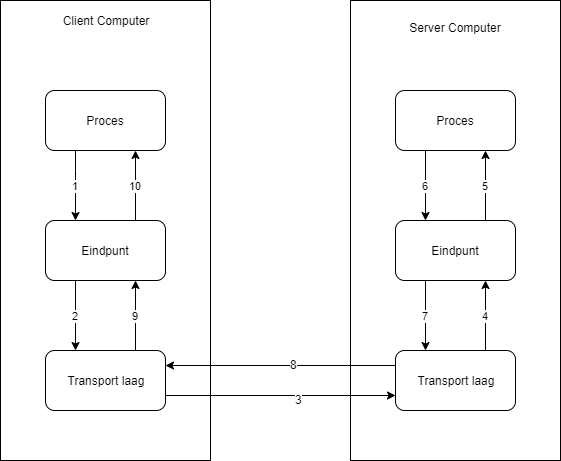
\includegraphics[width=12cm]{RPC-Diagram}
\end{center}
Sinds de concrete vaststelling van het RPC concept en vereisten in 1981 zijn er heel wat populaire uitvoeringen naar boven gekomen zoals  Apache's Avro (https://avro.apache.org/) in 2009, Google's gRPC (https://grpc.io/) in 2016 en Apache's Thrift (https://thrift.apache.org/) in 2019. Uit deze literatuurstudie blijkt spijtig genoeg dat er geen vergelijkend onderzoek gevoerd werd tussen verschillende RPC frameworks.
\section{gRPC}
Het gRPC framework is Google zijn eigen open source, performante en universele RPC framework. Voor maart 2015 gebruikte Google het Stubby RPC framework voor grootschalige communicatie, maart 2015 werd dit programma beschikbaar voor iedereen onder het open source project genaamd gRPC. 
%(https://cloud.google.com/blog/products/gcp/grpc-a-true-internet-scale-rpc-framework-is-now-1-and-ready-for-production-deployments)
Vandaag de dag wordt gRPC door een tal internetgiganten gebruikt waaronder Netflix en Cisco.
Het gRPC framework is gemaakt met performantie en gemak in gedachten, het maakt verbinden, bedienen en debuggen van gedistribueerde gemakkelijker. Ook zorgt gRPC voor zaken zoals data serialisatie, efficiënte netwerk communicatie, authenticatie en toegangscontrole. Er zijn enkele features en pluspunten dat gRPC laat uitblinken. Een van deze positieve punten is het grote aantal officieel ondersteunde talen, het ondersteund 10 populaire talen waaronder C\#, C++, Java, NodeJS, PHP en Python. Er werden geen artikelen gevonden die gRPC met andere frameworks vergelijken of die performantie van de ondersteunde talen testen.

Een pluspunt dat niet specifiek is aan gRPC maar toch vermeld mag worden is het gebruik van Google's Protobuf, een  taal ontwikkel voor het serialiseren van gestructureerde data (zie sectie 2.3).\\
Het meest onderscheidende feature van gRPC is de mogelijkheid voor bi-directionele communicatie door middel van http/2 (zie sectie 2.4).

\section{NodeJS}
In 1995, zeven jaar na de geboorte van het wereldwijd web, kwam JavaScript zijn eerste versie uit onder de naam 'Mocha'. De taal JavaScript, kortweg JS, is een programmeertaal dat je toelaat om allerlei complexe en/of interactieve elementen te implementeren op een webpagina. Denk dan maar aan cookies die je activiteit doorsturen of het live updaten van je chatvenster. De procesverwerking voor zulke JS taken gebeurt namelijk in de browser van jouw computer. Rond het jaartal 2009 was er een grote nood server-side JavaScript omgevingen om zowel de browsers minder te belasten als allerlei nieuwe JS mogelijkheden te creëren. In 2009 kwam Ryan Dahl en zijn collega's met de eerste uitgave van het JS-runtime-omgeving, een omgeving gemaakt voor het uitvoeren van JS code, NodeJS gebouwd op Google Chrome's 'V8 JavaScript Engine'. Vandaag de dag is NodeJS werelds beroemdste JS-runtime-omgeving, een omgeving gemaakt voor het uitvoeren van JS code buiten een webbrowser.

Typescript is een open-source taal dat verder op JavaScript bouwt. Het 
\\werking
\section{.NET 5}
Microsofts .NET is een gratis open-source framework voor het ontwikkelen van verschillende soorten applicaties zoals webapplicaties, mobiele applicaties, videospellen, API en nog veel meer. Het is Microsofts cross-platform alternatief voor .NET Framework wat enkel voor het Windows platform dient. Het .NET framework biedt de mogelijkheid om gebruik te maken van de programmeertalen C\#, F\# en Visual Basic. In dit onderzoek zal C\# gebruikt worden voor het schrijven van het API.
\\werking

Er worden twee API's gebruikt in dit onderzoek, beiden maken gebruik van een verschillend framework en programmeertaal. 
De twee API's die gebruikt worden zijn NodeJS geschreven in Typescript en .NET 5 geschreven in C\#.

\section{..}
bespreken van ..

\section{BS}
Je verwijst bij elke bewering die je doet, vakterm die je introduceert, enz. naar je bronnen. In \LaTeX{} kan dat met het commando \texttt{$\backslash${textcite\{\}}} of \texttt{$\backslash${autocite\{\}}}. Als argument van het commando geef je de ``sleutel'' van een ``record'' in een bibliografische databank in het Bib\LaTeX{}-formaat (een tekstbestand). Als je expliciet naar de auteur verwijst in de zin, gebruik je \texttt{$\backslash${}textcite\{\}}.
Soms wil je de auteur niet expliciet vernoemen, dan gebruik je \texttt{$\backslash${}autocite\{\}}. In de volgende paragraaf een voorbeeld van elk.

\textcite{Knuth1998} schreef een van de standaardwerken over sorteer- en zoekalgoritmen. Experten zijn het erover eens dat cloud computing een interessante opportuniteit vormen, zowel voor gebruikers als voor dienstverleners op vlak van informatietechnologie~\autocite{Creeger2009}.
%%=============================================================================
%% Methodologie
%%=============================================================================

\chapter{\IfLanguageName{dutch}{Methodologie}{Methodology}}
\label{ch:methodologie}

%% TODO: Hoe ben je te werk gegaan? Verdeel je onderzoek in grote fasen, en
%% licht in elke fase toe welke stappen je gevolgd hebt. Verantwoord waarom je
%% op deze manier te werk gegaan bent. Je moet kunnen aantonen dat je de best
%% mogelijke manier toegepast hebt om een antwoord te vinden op de
%% onderzoeksvraag.

\lipsum[21-25]



% Voeg hier je eigen hoofdstukken toe die de ``corpus'' van je bachelorproef
% vormen. De structuur en titels hangen af van je eigen onderzoek. Je kan bv.
% elke fase in je onderzoek in een apart hoofdstuk bespreken.

%\input{...}
%\input{...}
%...

%%=============================================================================
%% Conclusie
%%=============================================================================

\chapter{Conclusie}
\label{ch:conclusie}

% TODO: Trek een duidelijke conclusie, in de vorm van een antwoord op de
% onderzoeksvra(a)g(en). Wat was jouw bijdrage aan het onderzoeksdomein en
% hoe biedt dit meerwaarde aan het vakgebied/doelgroep? 
% Reflecteer kritisch over het resultaat. In Engelse teksten wordt deze sectie
% ``Discussion'' genoemd. Had je deze uitkomst verwacht? Zijn er zaken die nog
% niet duidelijk zijn?
% Heeft het onderzoek geleid tot nieuwe vragen die uitnodigen tot verder 
%onderzoek?

%\lipsum[76-80]



%%=============================================================================
%% Bijlagen
%%=============================================================================

\appendix
\renewcommand{\chaptername}{Appendix}

%%---------- Onderzoeksvoorstel -----------------------------------------------

\chapter{Onderzoeksvoorstel}

Het onderwerp van deze bachelorproef is gebaseerd op een onderzoeksvoorstel dat vooraf werd beoordeeld door de promotor. Dat voorstel is opgenomen in deze bijlage.

% Verwijzing naar het bestand met de inhoud van het onderzoeksvoorstel
%---------- Inleiding ---------------------------------------------------------

\section{Introductie} % The \section*{} command stops section numbering
\label{sec:introductie}

Hier introduceer je werk. Je hoeft hier nog niet te technisch te gaan.

Je beschrijft zeker:

\begin{itemize}
  \item de probleemstelling en context
  \item de motivatie en relevantie voor het onderzoek
  \item de doelstelling en onderzoeksvraag/-vragen
\end{itemize}

%---------- Stand van zaken ---------------------------------------------------

\section{State-of-the-art}
\label{sec:state-of-the-art}

Hier beschrijf je de \emph{state-of-the-art} rondom je gekozen onderzoeksdomein. Dit kan bijvoorbeeld een literatuurstudie zijn. Je mag de titel van deze sectie ook aanpassen (literatuurstudie, stand van zaken, enz.). Zijn er al gelijkaardige onderzoeken gevoerd? Wat concluderen ze? Wat is het verschil met jouw onderzoek? Wat is de relevantie met jouw onderzoek?

Verwijs bij elke introductie van een term of bewering over het domein naar de vakliteratuur, bijvoorbeeld~\autocite{Doll1954}! Denk zeker goed na welke werken je refereert en waarom.

% Voor literatuurverwijzingen zijn er twee belangrijke commando's:
% \autocite{KEY} => (Auteur, jaartal) Gebruik dit als de naam van de auteur
%   geen onderdeel is van de zin.
% \textcite{KEY} => Auteur (jaartal)  Gebruik dit als de auteursnaam wel een
%   functie heeft in de zin (bv. ``Uit onderzoek door Doll & Hill (1954) bleek
%   ...'')

Je mag gerust gebruik maken van subsecties in dit onderdeel.

%---------- Methodologie ------------------------------------------------------
\section{Methodologie}
\label{sec:methodologie}

Hier beschrijf je hoe je van plan bent het onderzoek te voeren. Welke onderzoekstechniek ga je toepassen om elk van je onderzoeksvragen te beantwoorden? Gebruik je hiervoor experimenten, vragenlijsten, simulaties? Je beschrijft ook al welke tools je denkt hiervoor te gebruiken of te ontwikkelen.

%---------- Verwachte resultaten ----------------------------------------------
\section{Verwachte resultaten}
\label{sec:verwachte_resultaten}

Hier beschrijf je welke resultaten je verwacht. Als je metingen en simulaties uitvoert, kan je hier al mock-ups maken van de grafieken samen met de verwachte conclusies. Benoem zeker al je assen en de stukken van de grafiek die je gaat gebruiken. Dit zorgt ervoor dat je concreet weet hoe je je data gaat moeten structureren.

%---------- Verwachte conclusies ----------------------------------------------
\section{Verwachte conclusies}
\label{sec:verwachte_conclusies}

Hier beschrijf je wat je verwacht uit je onderzoek, met de motivatie waarom. Het is \textbf{niet} erg indien uit je onderzoek andere resultaten en conclusies vloeien dan dat je hier beschrijft: het is dan juist interessant om te onderzoeken waarom jouw hypothesen niet overeenkomen met de resultaten.



%%---------- Andere bijlagen --------------------------------------------------
% TODO: Voeg hier eventuele andere bijlagen toe
%\input{...}

%%---------- Referentielijst --------------------------------------------------

\printbibliography[heading=bibintoc]

\end{document}
